\documentclass[titlepage, 12pt]{article}

\usepackage{framed}
\usepackage{enumitem}
\usepackage{geometry}
\geometry{
  letterpaper,
  margin=1in,
}

\usepackage{graphicx}
\graphicspath{{./images/}}
\usepackage{float}
\usepackage{subcaption}
\usepackage{amssymb}

\title{SE 2XB3 Group 4 Report 5}
\author{
  Huang, Kehao \\
  400235182 \\
  \texttt{huangk53@mcmaster.ca} \\
  L01
  \and
  Jiao, Anhao \\
  400251837 \\
  \texttt{jiaoa3@mcmaster.ca} \\
  L01
  \and
  Ye, Xunzhou \\
  400268576 \\
  \texttt{yex33@mcmaster.ca} \\
  L01
}
\date{26 February 2021}

\begin{document}
\maketitle{}

\newpage{}

\section{Building Heaps}
\label{sec:build}

\subsection{Estimations}
\label{sec:estimate}

\begin{description}
\item[\texttt{build\_heap\_1}] A loose upper bound is easy to establish since
  \texttt{sink} is \(\mathcal{O}(\lg{n})\) and less than \(n\) nodes are
  non-leaf nodes. Therefore, this algorithm takes at most
  \(\mathcal{O}(n\lg{n})\). However, to develop a tight upper bound, notice that
  different \texttt{sink} calls operate on ``mini-heaps'' of different \(n\).
  For example, for the first non-leaf node, the height, or \(\lg{n}\), of the
  heap containing this node and it children is only 1. The complexity of all
  \texttt{sink} operations on a heap with \(n\) non-leaf nodes can be expressed
  as the sum of a series:
  \begin{displaymath}
    \sum_{h = 0}^{\lg{n}} 2^h (\lg{n} - h) = 2n - \lg{n} - 2
  \end{displaymath}
  Each level of height \(h\) has at most \(2^h\) nodes. Sinking each node on the
  \(h\)th level takes at most \(\lg{n} - h\) swaps. Therefore, the tight bound
  of \texttt{build\_heap\_1} is concluded to be \(\mathcal{O}(n)\).
\item[\texttt{build\_heap\_2}] Assume appending a node to the bottom of the heap
  takes the amortized time \(\mathcal{O}(1)\). The complexity of the
  \texttt{insert} operation is the complexity of
  \texttt{bubble\_up}/\texttt{swim}, \(\mathcal{O}(\lg{n})\). Since \(n\) nodes
  would be inserted to build the heap, a loose upper bound of this heap building
  algorithm is \(\mathcal{O}(n\lg{n})\).
\item[\texttt{build\_heap\_3}] One round of calling
  \texttt{sink}/\texttt{heapify} on every node has complexity of
  \(\mathcal{O}(\lg{n})\) \texttt{sink} operations times n nodes,
  \(\mathcal{O}(n\lg{n})\). Each round of \texttt{sink} operations is able to
  move a node up only one level in the heap. In the worst case, for the actual
  root (maximum/minimum) of the heap to travel from the bottom level to the top
  level, \(\lg{n}\) (the height of the heap) rounds of \texttt{sink} operations
  are required. Though there is also a helper function \texttt{is\_heap} in each
  round of the \(n\) \texttt{sink} operations, contributing a \(\mathcal{O}(n)\)
  complexity to \texttt{build\_heap\_3}, it is on a smaller scale compared to
  the complexity of the \texttt{sink} operations. Thus, the expected complexity
  of this heap building algorithm is \(\mathcal{O}(n (\lg{n})^2)\).
\end{description}

\subsection{Experiments}
\label{sec:experiment}

The results of empirical timing experiments was unexpected.
\texttt{build\_heap\_2} was surprisingly slow. The run time of
\texttt{build\_heap\_2} was around the order of \(10^{-4}\) while the others were
of the order \(10^{-7}\). The different is so large that the scatter plots of the
other algorithms were suppressed down to a straight line when plotted along with
\texttt{build\_heap\_2}, as shown in Figure \ref{fig:comp}.

\begin{figure}[h]
  \centering
  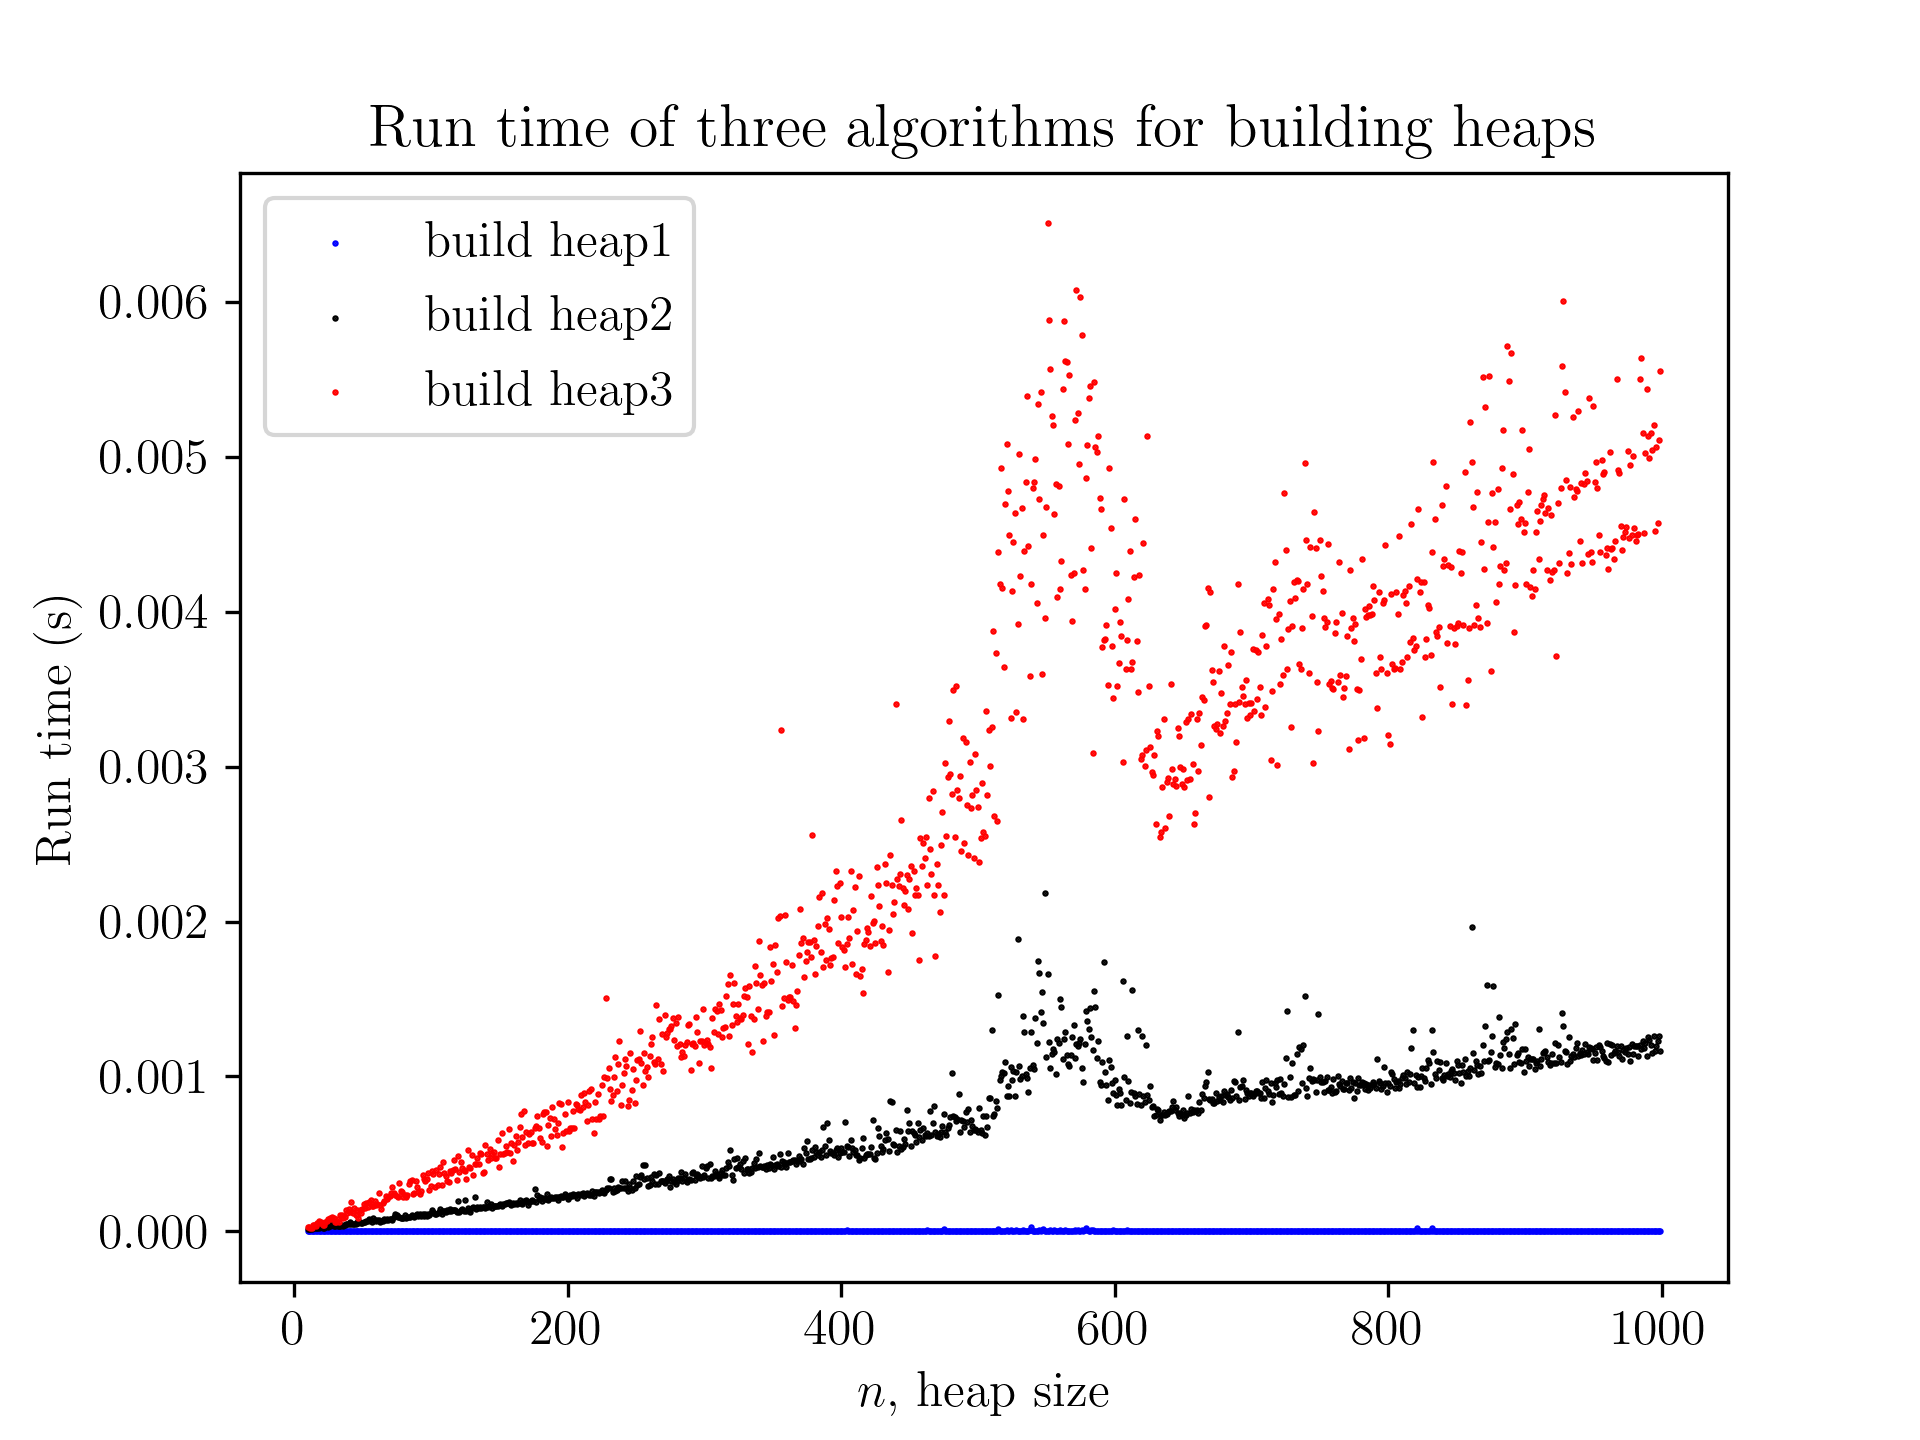
\includegraphics[width=\linewidth]{heap-comparison} 
  \caption{Heap building algorithms comparison}
  \label{fig:comp}
\end{figure}

The plotted data for both \texttt{build\_heap\_1} (in Figure \ref{fig:build1})
and \texttt{build\_heap\_3} (in Figure \ref{fig:build3}) is rather unstable.
Even though we tried to mitigate the effects of undesired factors like system
resources reallocation by running multiple tests on one input size and take the
fastest run time as the result for the input size, the regressions modeled with
our estimation did not fit well with the data.
\begin{figure}[h]
  \centering
  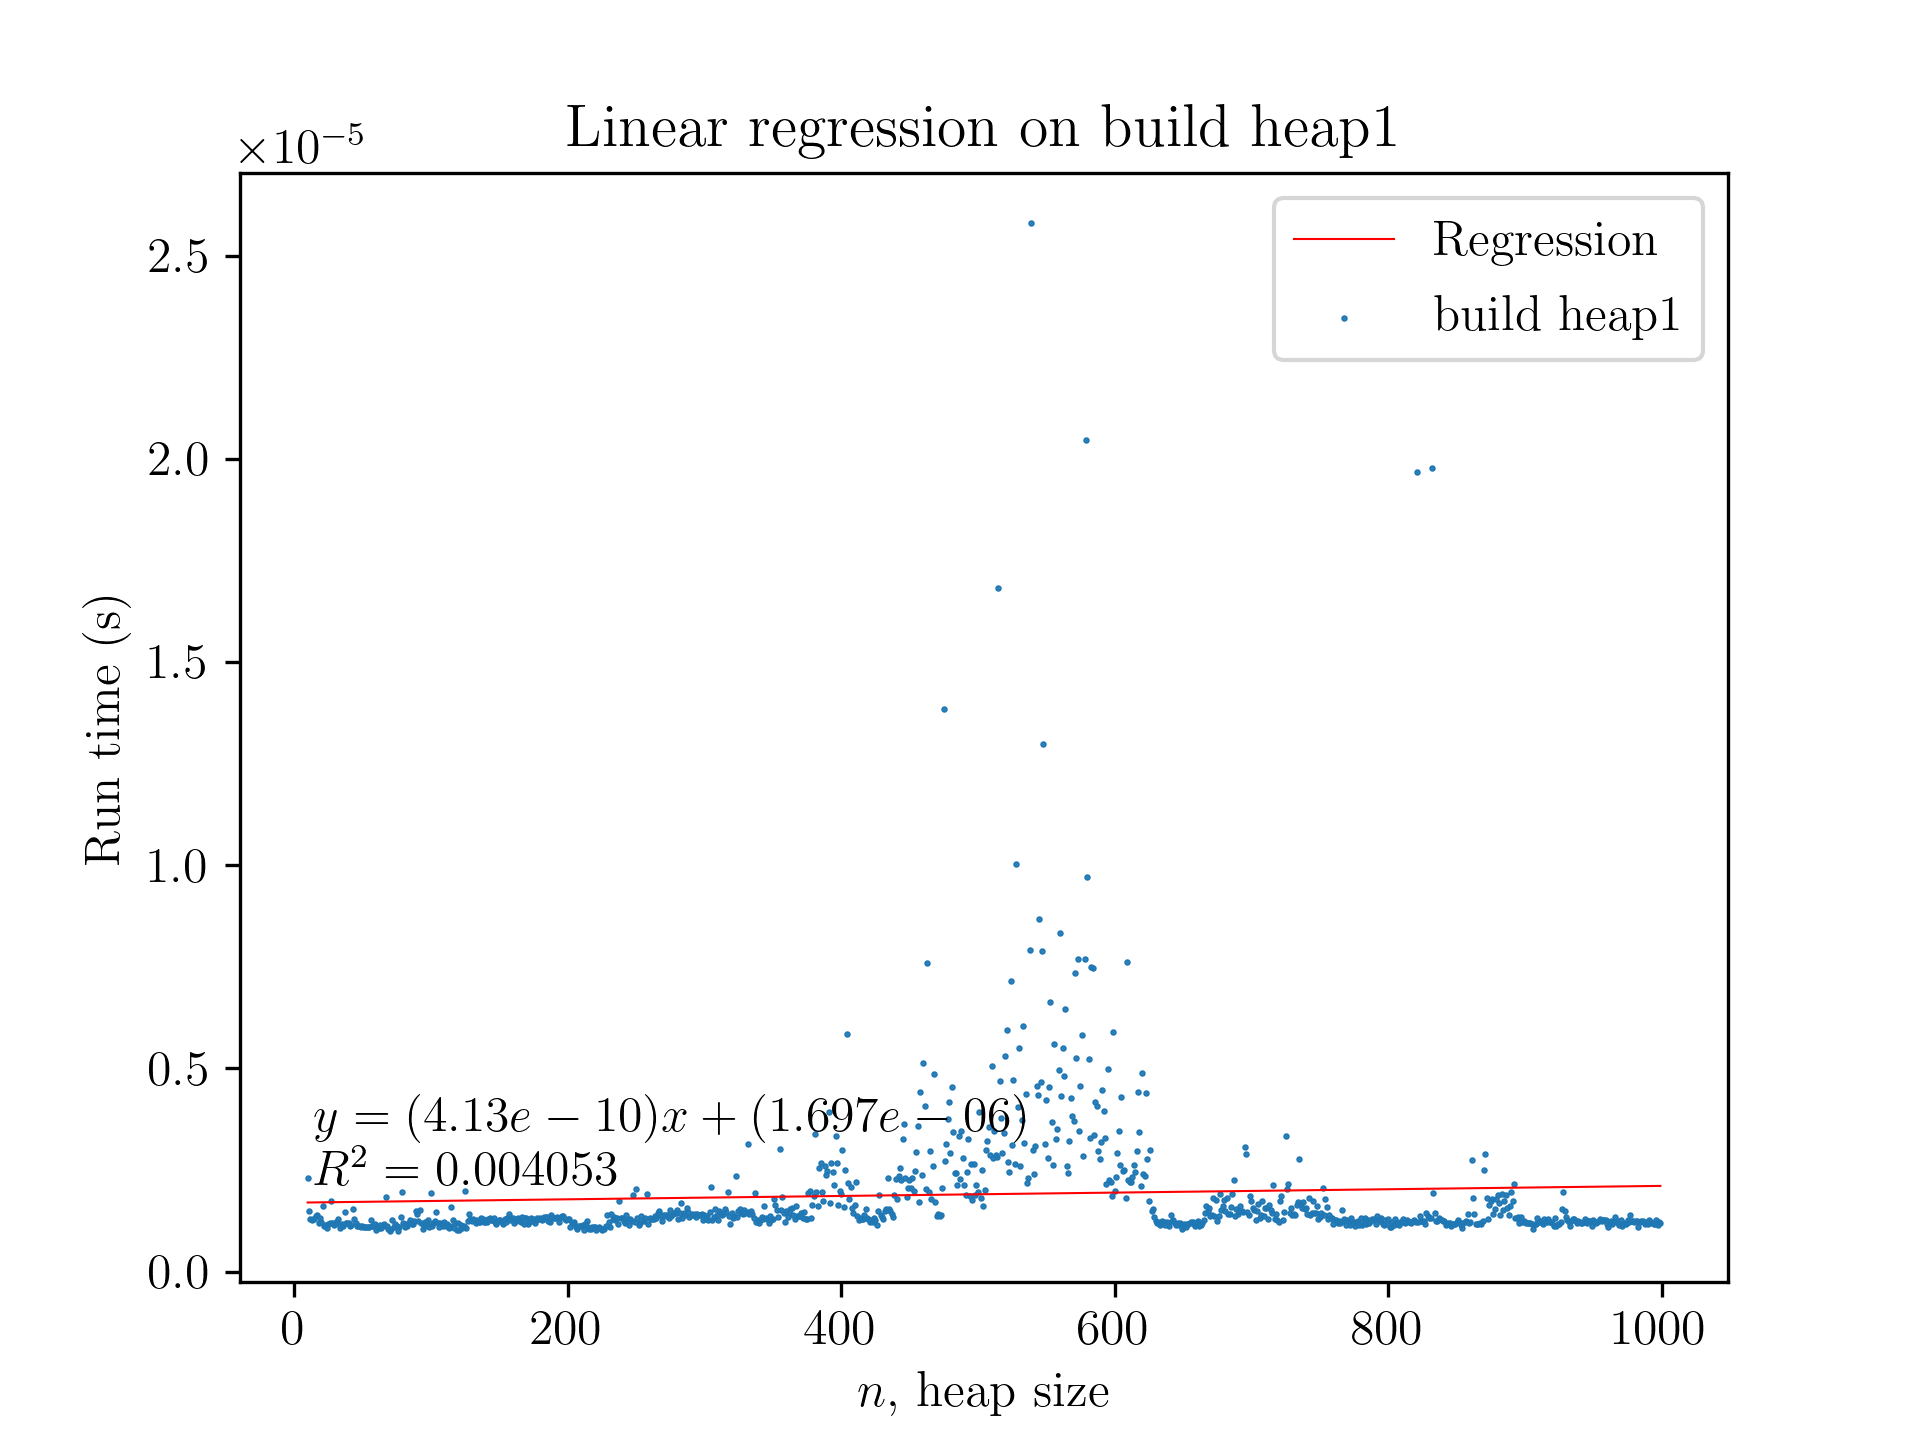
\includegraphics[width=\linewidth]{build1} 
  \caption{\texttt{build\_heap\_1} run time}
  \label{fig:build1}
\end{figure}
\begin{figure}[h]
  \centering
  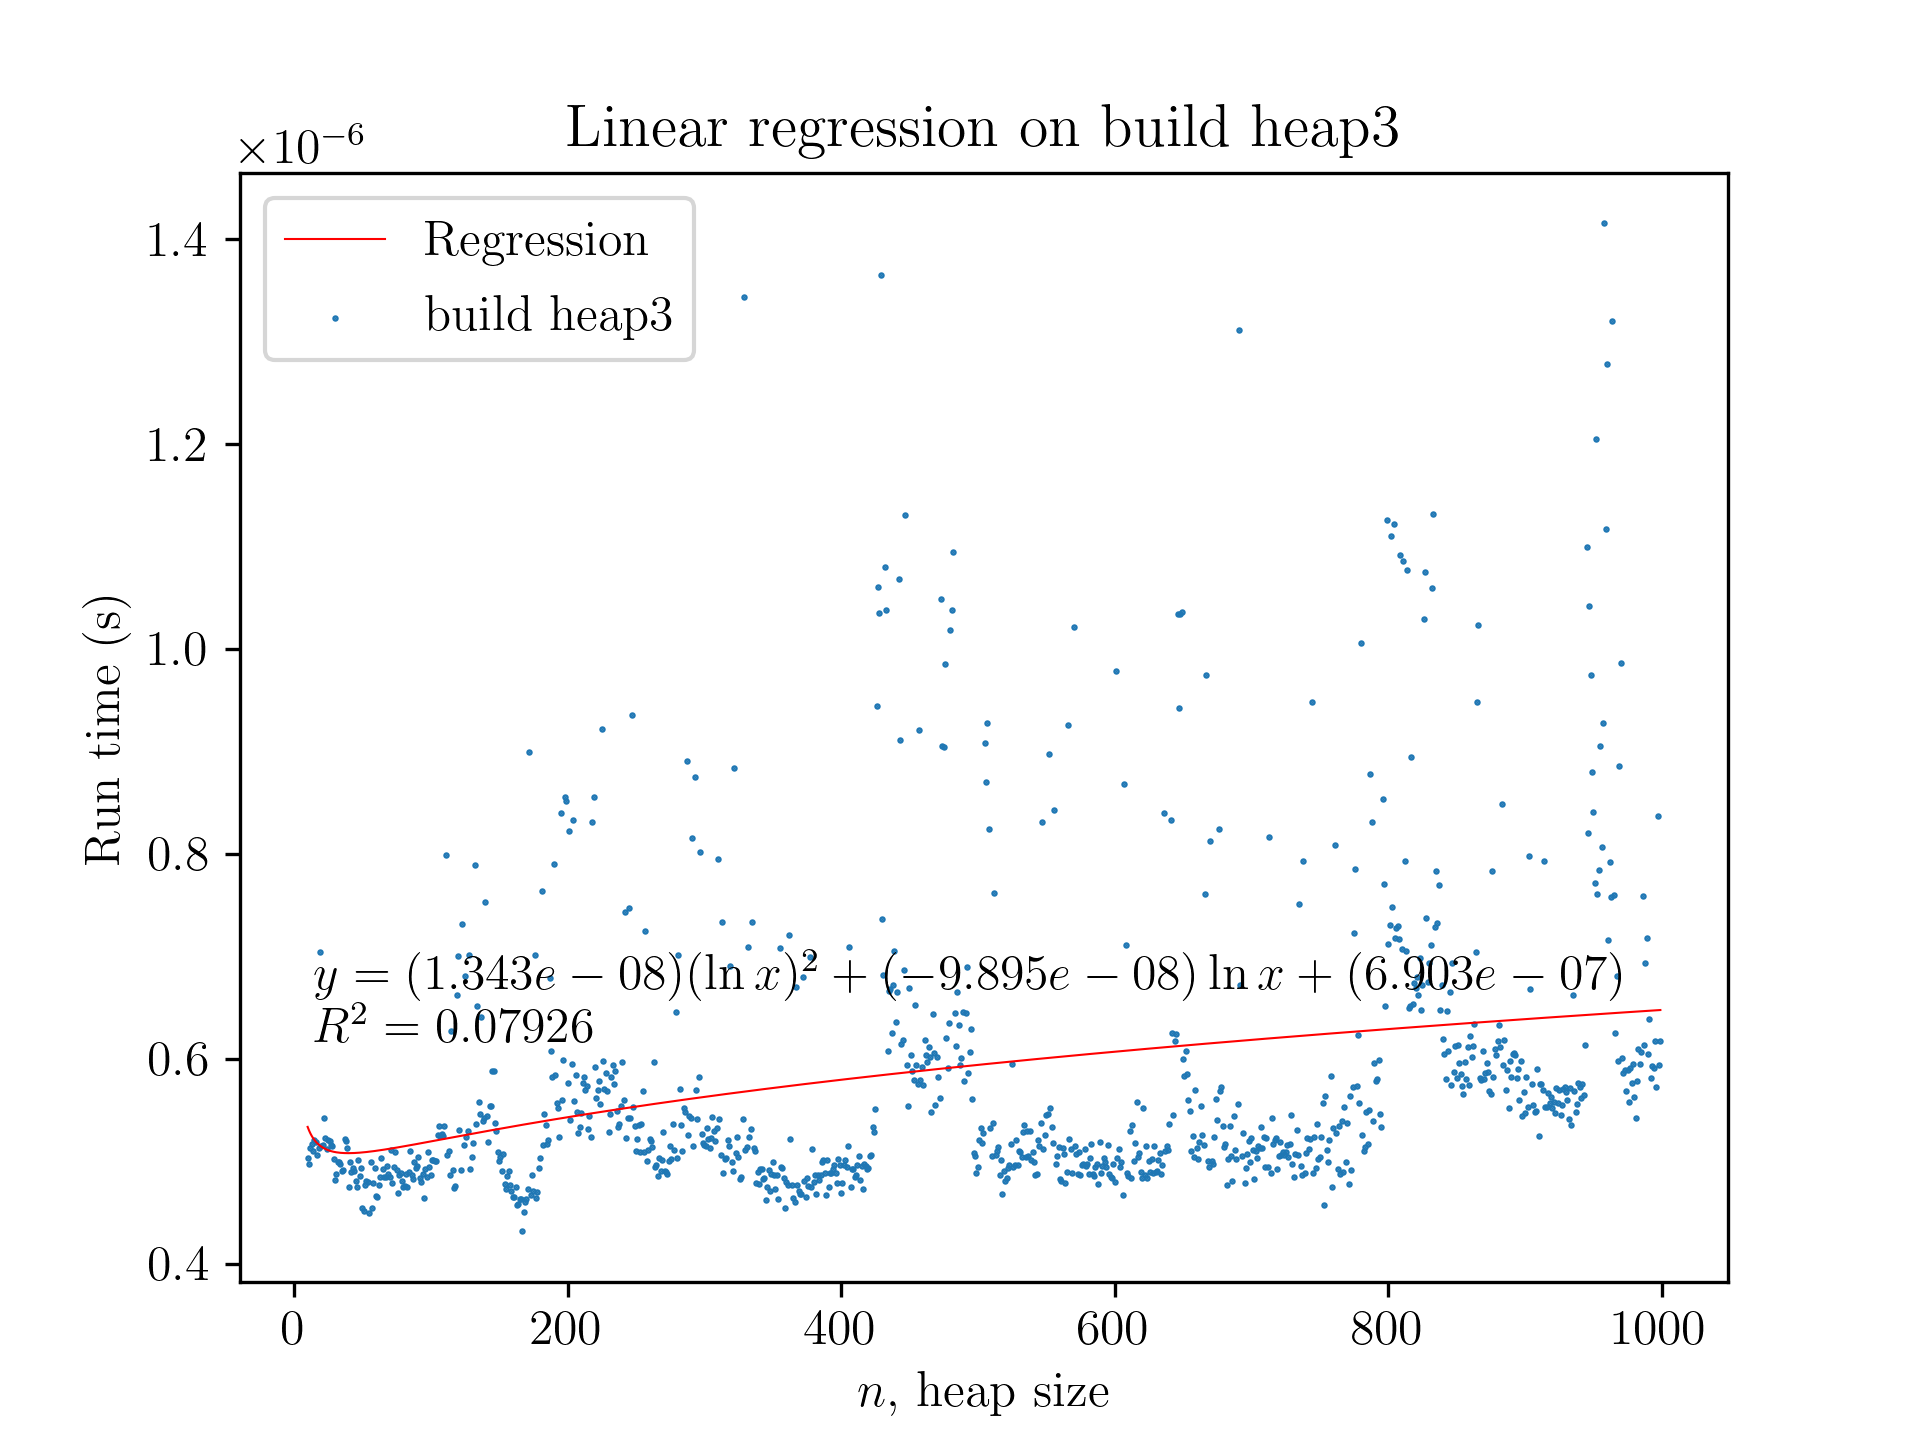
\includegraphics[width=\linewidth]{build3} 
  \caption{\texttt{build\_heap\_3} run time}
  \label{fig:build3}
\end{figure}

As for \texttt{build\_heap\_2} (in Figure \ref{fig:build2}), the data suggested
a linear growth. This is also different from our prediction. One of the proposed
reason is that inserting a list of elements into an empty heap is essentially
copying an array, along with the \texttt{bubble\_up} operation. In empirical
timing, the copying or appending action is a lot slower than the element
swapping involved in the \texttt{bubble\_up} operation. Therefore, the
\(\mathcal{O}(n)\) copying complexity dominates the empirical run time because
its run time is at a lower magnitude.
\begin{figure}[h]
  \centering
  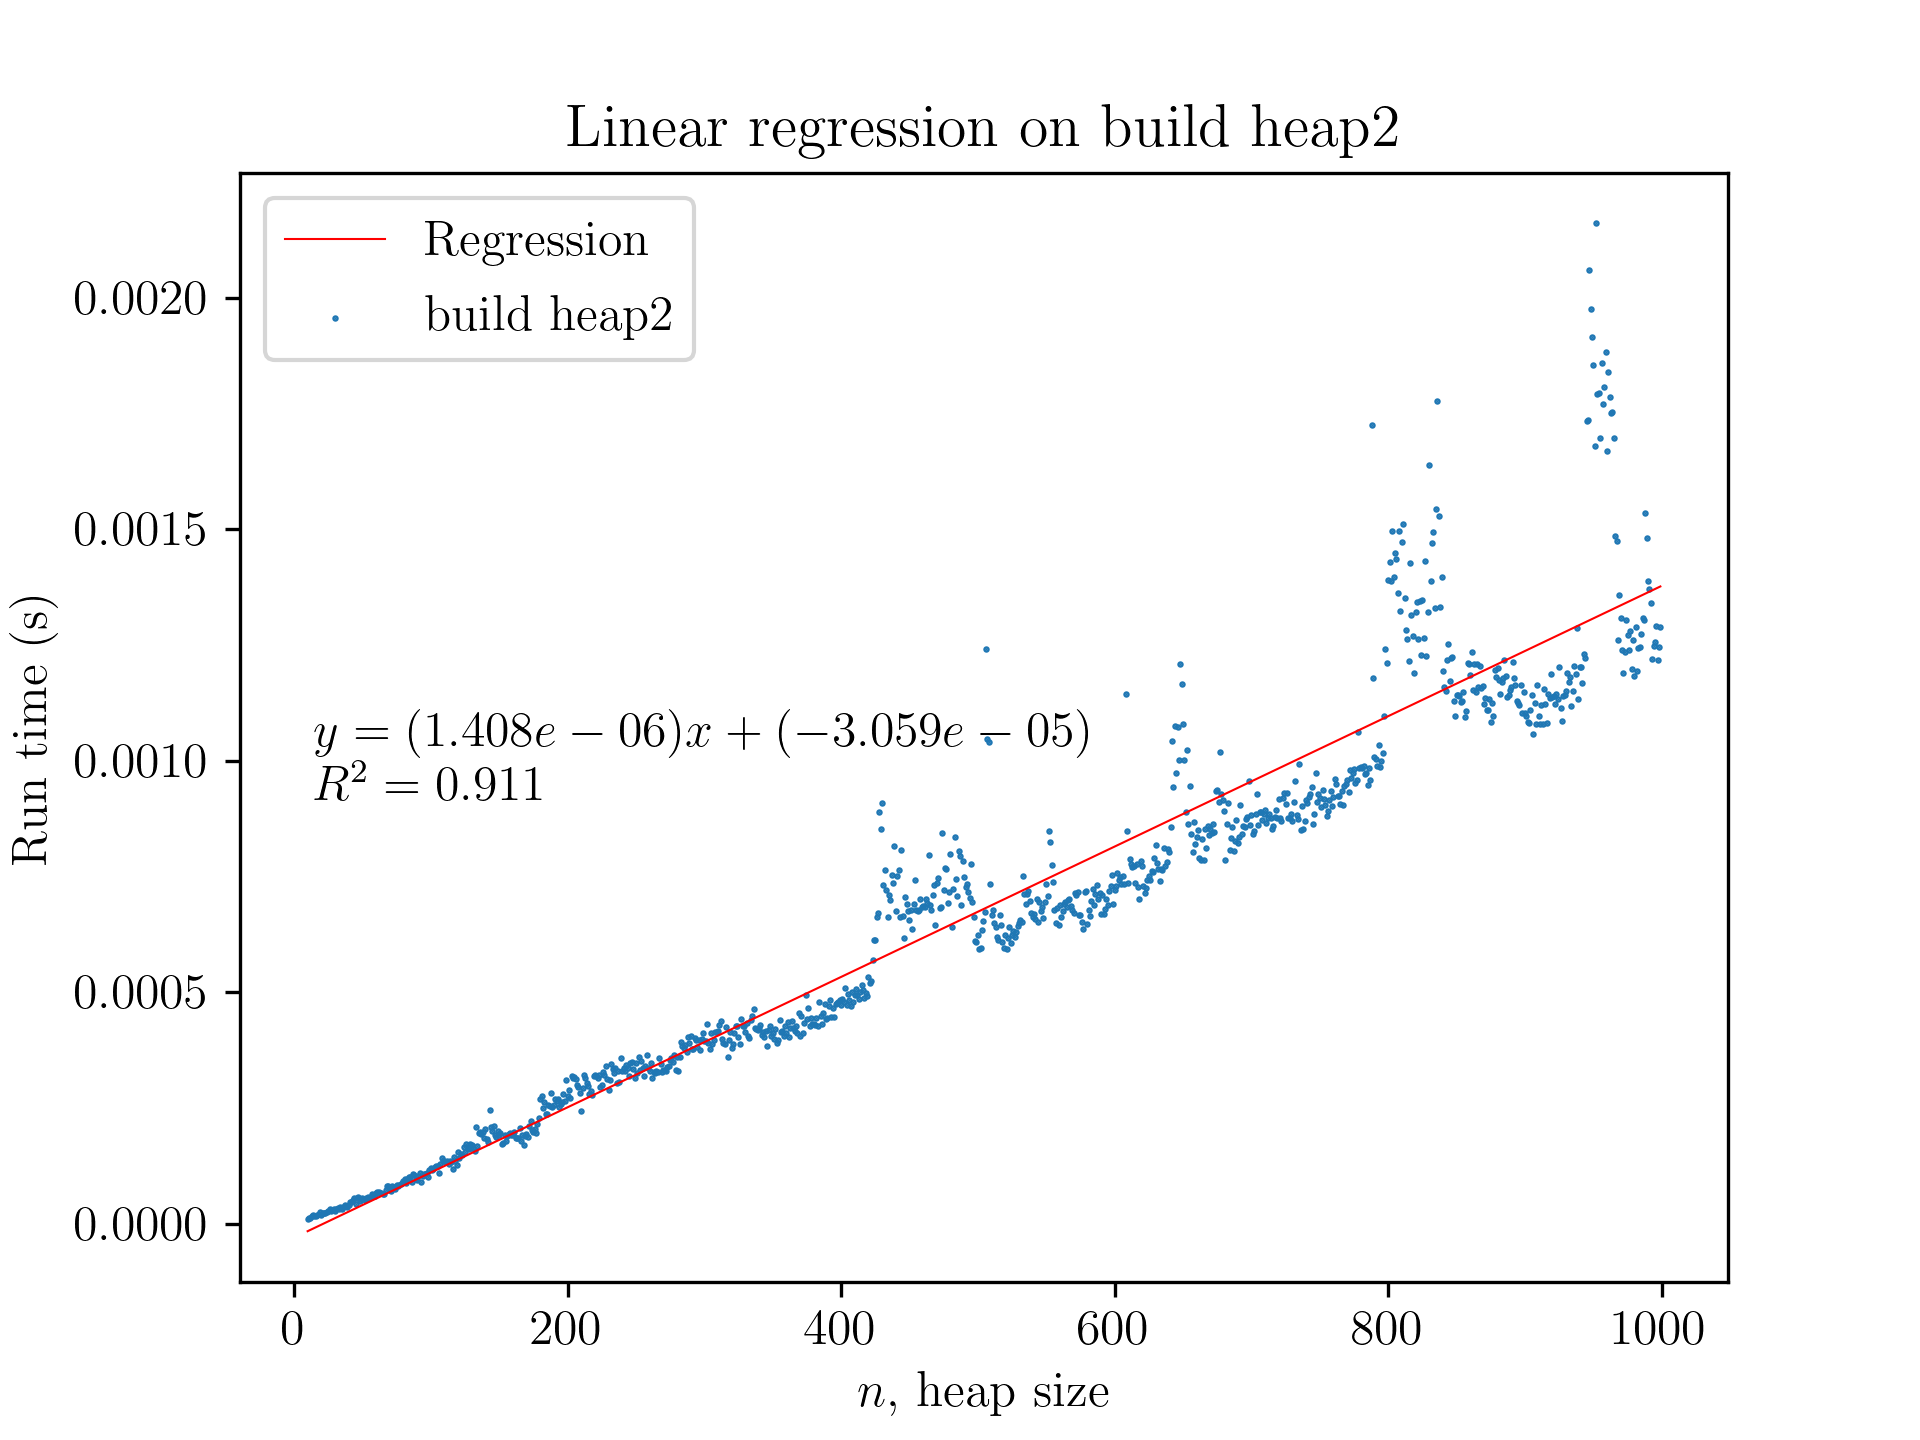
\includegraphics[width=\linewidth]{build2} 
  \caption{\texttt{build\_heap\_2} run time}
  \label{fig:build2}
\end{figure}

\subsection{\texttt{build\_heap\_3} Improvement}
\label{sec:inprove}

The depth of the heap causes the poor performance. If the larger elements are at
the bottom of the heap, we would need to heapify the nodes multiple times to get
the heap structure. The number of heapifying depends on the depth of the heap.

Improvement: Decreasing the depth of the heap can reduce the number of
heapifies. The more children each node can obtain, the shallower the heap depth
would be. In this way we could minimize the number of times moving the biggest
elements from bottom to top. Consequently, the performance of
\texttt{build\_heap\_3} will be improved.

\section{\(k\)-Heap}
\label{sec:kheap}

The asymptotic complexity of \texttt{sink} is believed to be \(\mathcal{O}(k
\log_{k}{n})\). In a \(k\)-heap, the nodes are organized in a complete \(k\)-ary
tree of height \(\log_{k}{n}\). In the worst case, a node \(e\), needs to “sink”
through \(\log_{k}{n}\) levels. On each level, \(k\) comparisons are required to
find the maximum element on the level. The maximum would then be swapped with
node \(e\). Hence, the complexity of \texttt{sink} is \(k\) comparisons times
\(\log_{k}{n}\) levels, \(\mathcal{O}(k \log_{k}{n})\).

A \(k\)-heap is essentially a \(k\)-ary tree. The height of a \(k\)-ary tree is
\(\log_{k}{n}\), which is smaller than that of a binary tree (heap), \(\lg{n}\).
The \texttt{swim} operation on a \(k\)-ary heap is \(\mathcal{O}(\log_{k}{n})\).
On the other hand, a larger \(k\) results in requiring more comparisons for
\texttt{sink} on each level of the tree. Therefore, in cases where applications
depending solely on the \texttt{swim} operation are prioritized over all other
operations, \(k\)-heaps of a large \(k\) have a huge advantage over binary
heaps. In other cases where \texttt{sink} or both \texttt{swim} and
\texttt{sink} are heavily used, such as Heapsort, \(k\)-heaps of any \(k\) are
not significantly better than binary heaps. In fact, the function family \(y =
k\log_{k}{x}\) minimizes for \(k \in \mathbb{N}\) at \(k = 3\), which means
3-ary heap is better than binary heap in most aspects, and any \(k\)-heap of \(k
> 3\) trades off its \texttt{sink} performance for that of \texttt{swim}.


\end{document}
